\subsection{Bridging induction}

Effective treatment of (quantifier-free) equality is one of the things that made SMT solvers and the Nelson-Oppen method successful.
When it comes to reasoning by induction, it has been investigated and addressed more thoroughly in the proof theory-oriented field.
SMT solvers are very much anchored in first-order logic, with several extensions on top of the core procedure supporting the use of induction principles.
Generally speaking, these add-on procedures require instantiating an induction scheme up front, as the choice of induction scheme to employ influence the first-order encoding of the query to the underlying SMT.
ATPs enjoy a greater degree of freedom, since they are able to apply an induction principle at any point during proof search, by inspecting the current state of the proof.
Cyclic proof systems provide yet more freedom, allowing to apply induction ``in hindsight'', based on further inference steps.

A long-standing problem in this area is that of choosing an appropriate \emph{induction hypothesis}.
Oftentimes, and depending on the form of induction principle being employed, a proof goal has to be \emph{strengthened} to make the induction step go through.
This is most apparent in software verification tasks that involve loops:
Induction is done on the number of loop iterations performed, and appropriate \emph{loop invariants} are required for this strategy to succeed.
Since software verification tools are, by and large, dominated by SMT solvers, automation of invariant inference has to come on top of the existing stack, as is done in Spacer~\cite{spacer} (and SeaHorn~\cite{seahorn}).

We would like to devise a framework that could facilitate both the more natural treatment of induction introduced by cyclic proof systems and the powerful loop invariant inference offered by IC3.
Loops are known to be a special case of (tail) recursion; however, they can also be treated elegantly using a simpler notion, that of \emph{transitive closure} (TC).
TC logics introduce atomic formulas of the form $\big(\mathrm{TC}_{x,y}\varphi\big)(s,t)$,
whose semantics is the existence of a path $s=u_0,u_1,\ldots,u_n=t$, $n\geq 1$, with $\varphi[u_i/x,u_{i+1}/y]$
holding between all pairs of successive elements.
$x$ and $y$ are supposed free variables in $\varphi$, so $\varphi$ is commonly thought of as representing a binary relation, and $\big(\mathrm{TC}_{x,y}\varphi\big)$ --- the (algebraic) transitive closure of this relation.
A commonly used variant is $\big(\mathrm{RTC}_{x,y}\varphi\big)$, with the only difference being that $n\geq 0$ (instead of $1$),
which in turn induces the \emph{reflexive} transitive closure.
Another extension allows relations of arbitrary even arities
$\big(TC_{x_1,\ldots,x_k,y_1,\ldots,y_k}\varphi\big)$;
this transitive closure can be thought of as a path between $k$-tuples, where $x_1,\ldots,x_k$ and $y_1,\ldots,y_k$ represent coordinates of adjacent tuples.
In the sequel, we use the phrase ``transitive closure'' as an umbrella term for these closely related variants.

\begin{proposal}Transitive closure is a convenient representation of inductive definitions that can be used to encompass both proof search and SMT-based invariant inference.
\end{proposal}


The proposal is to ingrain the notion of transitive closure in the language and proof search procedures of automated theorem provers.
In the spirit of the mechanics of SMT solvers, where different \emph{theory solvers} are combined using the Nelson-Oppen method,
we postulate that an important module would be a solver specifically capable of reasoning
about transitive closure properties.
Particularly, this solver will be able to construct models of quantifier-free
FO(TC) formulas (first-order formulas with TC).

\begin{researchquestion}How can TC logic make automated reasoning with induction more effective?
\end{researchquestion}

The first expected benefit is that TC enables clean, compact representation of data-related properties,
making the logic easier to use and the resulting formalisms clearer.
For example, the classical construction of the natural numbers from first principles involves a zero element and a successor operator.
Based on this definition, operations and relations over natural values, such as the order relation $\leq$, is defined recursively:
\[
\begin{array}{l@{\hspace{4em}}l}
\begin{array}[t]{l}
\rInductive~\tnat~\eqdef \\
\quad |~0 : \tnat \\
\quad |~S : \tnat \to\tnat
\end{array}
&
\begin{array}[t]{l}
\rInductive~\fle : \tnat \to \tnat \to \tProp ~\eqdef \\
\quad |~\fctorlen : \forall n:\tnat,~ \fle\,n\,n\\
\quad |~\fctorleS : \forall (n\,m:\tnat),~ \fle\,n\,m\to\fle\,n\,(S\,m)
\end{array}
\end{array}
\]

The definition of $\fle$ above is taken from the Coq standard library and is amongst the most basic ones in the Calculus of Inductive Constructions (CIC); yet it commonly baffles newcomers and takes some time convincing oneself that it indeed defines the familiar notion of $\leq$.
Using transitive closure, however, offers a more compelling formulation:
\[
\fle\,x\,y ~\eqdef~ \big(\RTC{x,y}\,S\,x=y\big)(x,y)
\]

The above formula reads: $x\leq y$ iff $y$ can be obtained from $x$ by zero or more application of $S$, the successor operator.
This naturally aligns with our fundamental perception of ordering of natural numbers.
In this sense, the transitive closure construct captures a recurring pattern in recursive definitions, one that seasoned logicians can identify at a glance, but which nevertheless adds some amount of unnecessary ``noise'' when constructing proofs.
This noise becomes more significant as definitions grow in complexity, and eventually encumbers proof development, especially proof automation.
In particular, chained application of a previously defined function or relation is so commonly useful, that it makes sense to define a designated notation for it:
\[
\fle\,x\,y ~\eqdef~ x[S^*]y \hspace{4em}
\textit{where:}~
\begin{array}[t]{l}
  {} [f] : D\to D\to\tProp ~\eqdef~ \lambda x\,y, f\,x=y \\
  {} [R^*] ~\eqdef~ \big(\RTC{x,y}\,R\,x\,y\big) \\
  {} [f^*] ~\eqdef~ \big[[f]^*\big]  \qquad\textrm{\small(\textit{and analogously for} ${[]}^+$)}
\end{array}
\]

The use of square brackets in notations occurring in this document helps to avoid ambiguous expressions, and also provides an opportunity for using binary relations as infix operators;
\eg, we write $x[S^*]y$ as a more elegant alternative to $[S^*]\,x\,y$.

\begin{figure}
\begin{center}
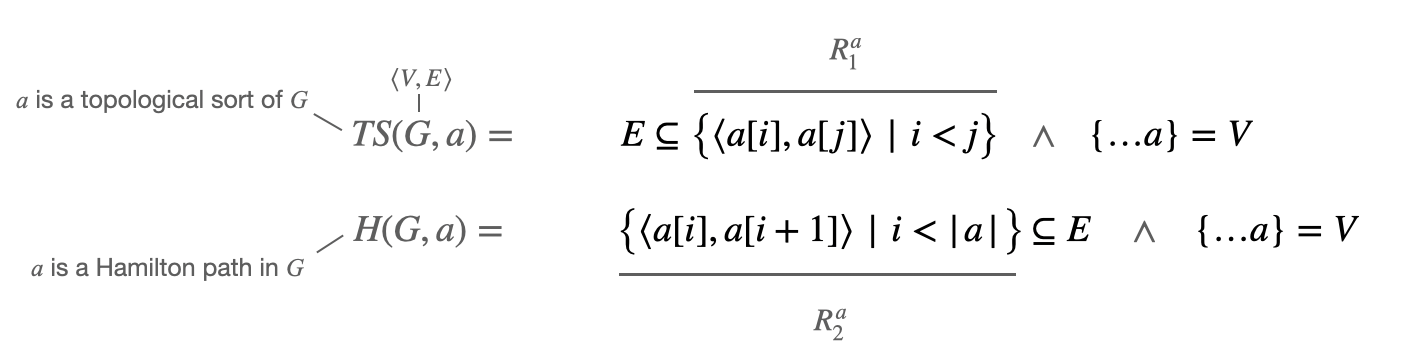
\includegraphics[width=.8\textwidth]{img/topological-and-hamilton.png}
\end{center}
\todo{typeset with $\fTS\,G\,a$ and $\fH\,G\,a$}
\caption{Formal definitions of topological sort and Hamilton paths
  for use in \autoref{plan:hamilton}.}
\label{plan:hamilton-defs}
\end{figure}

We argue that the compact TC formulation allows for shorter proofs --- which, in turn, lead to easier proof derivation processes in both interactive and fully-automated settings.
We use the following example to illustrate this point; it is a problem taken from an undergraduate class on algorithms and complexity theory.

\begin{example}~\label{plan:hamilton}
\begin{tabular}[t]{lp{10cm}}
\textit{Given:} & A directed acyclic graph $G=\langle V,E\rangle$.
\\
\textit{Task:}  & Determine whether the graph contains a \emph{Hamilton path}; \ie, a (directed) path that visits every $u\in V$ exactly once.
\end{tabular}

\medskip
This exercise is given following a lecture on DFS, BFS, and topological sort.
This gives rise to the following short solution:
(1)~Topologically sort the vertices of $G$;
(2)~Check whether the resulting array constitutes a path,
 that is, every two consecutive elements are connected by an edge.
 
While the algorithm looks simple, it is not at all obvious that it is correct w.r.t.\@ the requirements.
Clearly, if step (2) returns $\ftrue$, then it has correctly discovered a Hamilton path (even without considering any properties of topological sort).
But when the outcome is $\ffalse$, some acute reasoning is required to show that there does not exist a \emph{different} ordering of $V$ that corresponds to a Hamilton path.
To establish correctness, the student needs to formalize the definition of topological sort and that of a Hamilton path
(\autoref{plan:hamilton-defs}).
Then the following proof goal must be accomplished:
\begin{equation}\label{plan:hamilton-goal}
\fH\,G\,a,~\fTS\,G\,a' ~\vdash~ a = a'
\end{equation}

That is, in a DAG containing a Hamilton path, there is exactly one possible topological sort, and that sort is identical to the order imposed by the Hamilton path.
(Notice that a DAG may contain at most one Hamilton path; this property is obtained as a simple corrollary of (\ref{plan:hamilton-goal}).)

An insight into the proof can be offered by considering the two binary relations $R_1^a$, $R_2^a$ occurring in the definitions of $\fTS$ and $\fH$.
A keen observer may notice that: $R_1^a = [{R_2^a}^+]$.
The implication would be that the topological sort ($R_1^a$) is uniquely determined by the Hamilton path ($R_2^a$) if the latter exists.
From there, proving (\ref{plan:hamilton-goal}) is by no means trivial, but it does follow from rather standard algebraic properties:
\begin{enumerate}
  \item $R_1^a$ is a \underline{\emph{total order}} on $V=\{...a\}$.
  \item A total order is \underline{\emph{maximal w.r.t.\@ set inclusion}}
    over all (partial) orders on the same set.
  \item The mapping $a \mapsto R_1^a$ is \underline{\emph{injective}}.
\end{enumerate}

Notably, the monotonicity of the transitive closure operator $^+$ (as of any closure operator) is utilized here to establish the relationship $R_1^a \subseteq R_1^{a'}$.
In this small instance, it is completely reasonable to expect that an automated prover can infer the three auxiliary properties listed above, as well as construct their proofs, without the user's intervention.
In more complex scenarios, the aspiration is toward the prover and the user working hand-in-hand, with the prover suggesting some conjectures that can progress the proof, and the user selecting the ones that make the most sense while also adding propositions that were not automatically discovered.
The use of algebraic concepts here is deliberate: the phrases ``total order'', ``set inclusion'', ``injective mapping'' all encode knowledge previously gained from human experience in defining and solving mathematical problems.
\end{example}

\todo{describe the objective and how the transitive closure solver fits in the general scheme}

\begin{figure}
\begin{center}
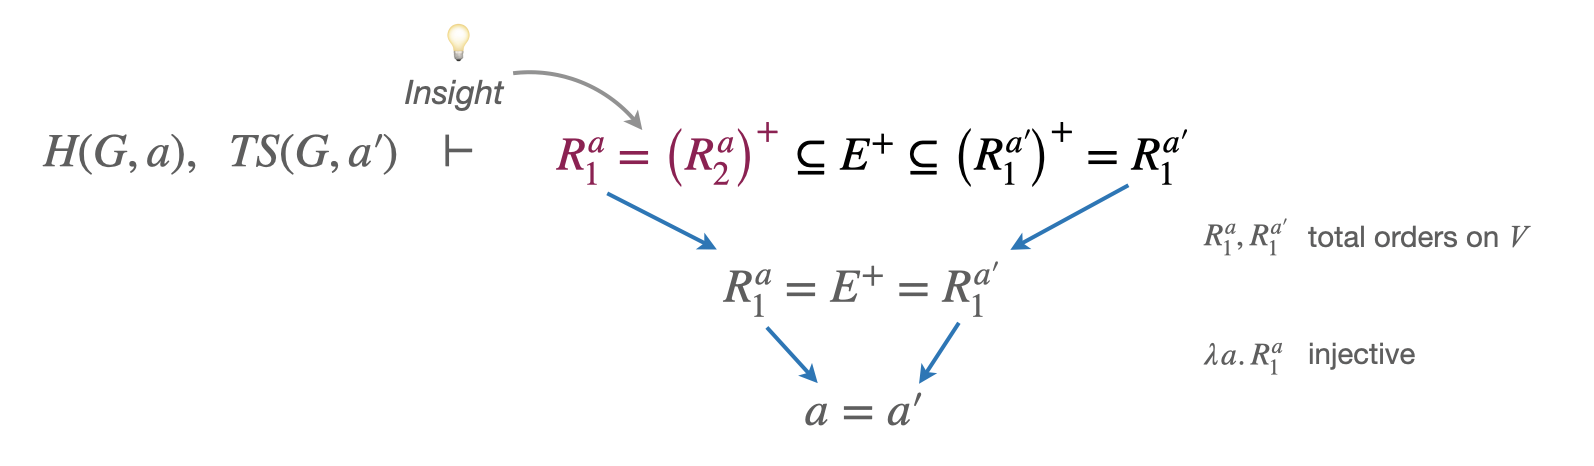
\includegraphics[width=.8\textwidth]{img/topological-and-hamilton-proof-sketch.png}
\end{center}
\vspace{-2em}
\todo{typeset with $\fTS\,G\,a$ and $\fH\,G\,a$}
\caption{A sketch of the proof described in \autoref{plan:hamilton}.}
\label{plan:hamilton-proof}
\end{figure}


\begin{researchquestion}How can we leverage the success of cyclic proof systems for automated reasoning in TC (and co-TC)?
\end{researchquestion}


\begin{researchquestion}How can we combine inductive and deductive reasoning for automatic inference of proper induction hypotheses?
\end{researchquestion}